\chapter{Design}
\label{ch:design}

This chapter defines our threat model, \ac{WASM} extension, and design to provide memory safety for programs compiled to \ac{WASM}.


\section{Threat Model}
\label{sec:threat-model}

In our threat model (\cref{fig:threat-model}), we differentiate between two aspects of memory safety.
In both models, we depict trusted components (marked with a \raisebox{-0.25em}{
\includegraphics[clip,height=1em]{./figures/build/trusted}}) in green and untrusted components (marked with a \raisebox{-0.25em}{
\includegraphics[clip,height=1em]{./figures/build/untrusted}}) in red.
We additionally highlight the component we are trying to harden (marked with a \raisebox{-0.25em}{
\includegraphics[clip,height=1em]{./figures/build/poi}}).

\begin{figure}
    \centering
    \begin{subfigure}[T]{0.45\textwidth}
        \centering
        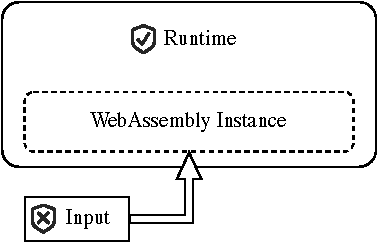
\includegraphics{figures/build/wasm-internal-mem-safety}
        \caption{Internal memory safety.}
        \label{fig:internal-mem-safety}
    \end{subfigure}
    \hfill
    \begin{subfigure}[T]{0.45\textwidth}
        \centering
        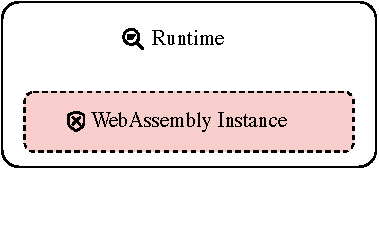
\includegraphics{figures/build/wasm-external-mem-safety}
        \hspace{\fill}
        \caption{External memory safety.}
        \label{fig:external-mem-safety}
    \end{subfigure}
    \caption{Threat model for internal and external memory safety.}
    \label{fig:threat-model}
\end{figure}

\begin{description}
    \item[Internal Memory Safety:] Ensures memory safety within the boundaries of a sandbox.
    Our point of view is from within a WebAssembly instance, we trust the runtime (and the host we are running on), but we do not trust external input (\cref{fig:internal-mem-safety}).
    \item[External Memory Safety:] Maintains the memory safety of the sandbox itself against potentially malicious programs.
    Our point of view is from the runtime; we trust the platform we are running on, but not the WebAssembly programs we are executing (\cref{fig:external-mem-safety}).
\end{description}

\subsection{Internal Memory Safety}
\label{subsec:internal-memory-safety}
For internal memory safety, the program within the sandbox and its runtime, including its compiler, are considered trusted and assumed to be bug-free.
Untrusted input (e.g., network data, file reads) originates from outside the sandbox and may be controlled by an attacker.
This model mirrors the threat environment of a standard non-\ac{WASM} program.
Potential threats include:

\begin{itemize}
    \item \textbf{Buffer overflows:} Attempts to access memory beyond allocated buffer boundaries.
    \item \textbf{Use-after-free:} Attempts to access deallocated memory.
\end{itemize}

\noindent
As discussed in \cref{sec:wasm}, WebAssembly's design inherently mitigates some threats common in non-\ac{WASM} environments, so we will not consider the following vectors:

\begin{itemize}
    \item \textbf{Return-oriented attacks:} {\ac{WASM}'s} structured control flow constructs prevent arbitrary code execution through stack manipulation.
    \item \textbf{Calling unknown function pointers:} Function tables enforce a strict mechanism for function calls, ensuring the integrity of call targets.
\end{itemize}

\subsection{External Memory Safety}
\label{subsec:external-memory-safety}

For external memory safety, we focus on the security of the sandbox.
Threats originate from running untrusted programs, which may be adversarial or buggy.

\begin{itemize}
    \item \textbf{Sandbox escapes:} Attempts to break out of the sandbox's restrictions and access host resources.
    \item \textbf{Side-channel attacks:} Exploiting timing differences or resource usage patterns to infer sensitive information.
\end{itemize}

\noindent
We assume that the operating system and underlying target architecture are free of bugs that malicious targets might exploit.
This does not include assumptions about potential spectre-like~\cite{kocher2020spectre} attacks.
The compiler needs to ensure that bounds checks are guarded against side-channel attacks.

Additionally, we do not consider exploits of the program running in the sandbox as vulnerabilities as long as they stay contained in the sandbox.


\section{Overview}
\label{sec:overview}

\begin{figure*}[t]
    \centering
    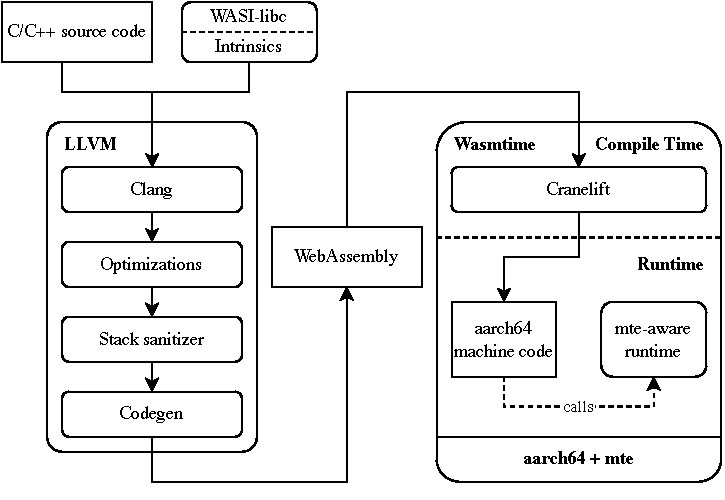
\includegraphics{figures/build/overview}
    \caption{Overview of the compilation and execution workflow.}
    \label{fig:overview}
\end{figure*}

Figure~\ref{fig:overview} presents an overview of our prototype.
At build time, the unmodified C/C++ sources and a modified version of libc are compiled using LLVM~\cite{lattner2004llvm}.
After optimizations, a stack sanitizer analyzes all functions and inserts instrumentation as necessary.
LLVM's backend then generates WebAssembly binaries that can be deployed and executed on various devices.


\section{WebAssembly Extension}
\label{sec:wasm-extension}

We designed an extension to WebAssembly that provides primitives to the modified standard library and the stack sanitizer to guarantee memory safety for selected allocations.
Our extension builds on wasm64, the 64-bit variant of WebAssembly.
We choose wasm64, because it uses a 64-bit integer index type, with 48 of those bits used to index memory.
This allows us to allocate and store up to 16 bits of metadata per pointer.

For our extension, we introduce the notion of abstract segments and tagged pointers.
We introduce three new instructions that allow the creation of abstract segments and tagged pointers from raw pointers.
These pointers carry provenance and can only access the segment they were created with.
Conversely, segments can only be accessed by the tagged pointer created with them rather than with raw indices without provenance.

\begin{equation*}
    \text{(new instructions) } e \Coloneqq \textbf{segment.new} \mid \textbf{segment.set\_tag} \mid \textbf{segment.free}
\end{equation*}

\paragraph{}
In the following paragraph, we describe the new instructions in detail.

\begin{description}
    \item[\texttt{segment.new}:] Create a new, zeroed memory segment.
    This instruction takes two arguments: a memory index and a size.
    The instruction generates a new tag, assigns it to the piece of memory, and returns a tagged pointer that can be used to access the segment.
    \item[\texttt{segment.set\_tag}:] This instruction takes a memory index, a length, and a tagged pointer and applies the tag from the tagged pointer to the memory segment located at the index with the passed length.
    This can be used to move ownership from one segment to another or to merge segments.
    \item[\texttt{segment.free}:] This instruction invalidates a segment by tagging the segment with a new, implementation-defined tag.
    This instruction takes two arguments: a memory index and a length.
    After this instruction, the tagged pointer being used to access the segment is no longer valid, and accessing the segment through it will result in a trap.
\end{description}

We also modify the semantics of existing load and store instructions.
They still take an integer as an index, but we introduce provenance to integers, which we can track at runtime using the unused 16 upper bits in pointers.
If a segment is accessed, the runtime will check that the tagged pointer is allowed to access the segment, i.e., the metadata matches the metadata created by the \texttt{segment.new} instruction.
If this is not the case, the runtime throws a trap.

At startup, the linear memory consists of a single segment that can be accessed using untagged indices, allowing unmodified code to run under our new semantics without modifications.
This design choice also allows the gradual integration of safety primitives into specific parts of WebAssembly applications where enhanced security is required.
For instance, it enables the introduction of a hardened malloc implementation, which prevents spatial and temporal safety bugs for heap-allocated memory.
Additionally, we can analyze stack allocations to only harden those accessed using untrusted indices or escape our analysis, e.g., by taking their address and passing it to another function.

\paragraph{Alignment}
All segments are aligned to 16 bytes, corresponding to the alignment of \ac{MTE} (see \cref{subsec:mte}).
This is an implementation choice that may be changed once we support additional implementations.
More details can be found in \cref{sec:future-work}.

\subsection{Typing Rules}
\label{subsec:typing}

In \cref{fig:typing-rules}, we extend the typing rules in the \ac{WASM} paper~\cite{haas2017bringing} in the notation of \citeauthor*{pierce2002types}~\cite{pierce2002types}.
The rules are of the form of $C \vdash e : \mathit{tf}$.
An instruction $e$ is valid under the context $C$, with $C_\text{memory}$ being used to access a context component, such as the memory.
The rule $C_\text{memory} = n$ ensures that the instruction can only be used when a memory is declared.
The rule $2^a=16$ ensures the alignment is 16\,bytes, as described in the previous section.
The type $\mathit{tf} = t_1^* \rightarrow t_2^*$ describes how the instruction manipulates the operand stack.
The instruction $e$ expects an operand stack where it pops off $t_1^*$ and pushes $t_2^*$.

\begin{figure}[t]
    \begin{prooftree}
        \AxiomC{$C_{\text{memory}} = n$}
        \AxiomC{$2^a=16$}
        \BinaryInfC{$C \vdash \textbf{segment.new}\ a\ o : \text{i64}\ \text{i64} \rightarrow \text{i64}$}
    \end{prooftree}
    \begin{prooftree}
        \AxiomC{$C_{\text{memory}} = n$}
        \AxiomC{$2^a=16$}
        \BinaryInfC{$C \vdash \textbf{segment.set\_tag}\ a\ o : \text{i64}\ \text{i64}\ \text{i64} \rightarrow \epsilon$}
    \end{prooftree}
    \begin{prooftree}
        \AxiomC{$C_{\text{memory}} = n$}
        \AxiomC{$2^a=16$}
        \BinaryInfC{$C \vdash \textbf{segment.free}\ a\ o : \text{i64}\ \text{i64} \rightarrow \epsilon$}
    \end{prooftree}
    \caption{Typing rules of the new instructions. For the definition of context $C$, see the \ac{WASM} paper~\cite{haas2017bringing}.}
    \label{fig:typing-rules}
\end{figure}

\subsection{Small-Step Reduction Rules}
\label{subsec:small-step-reduction-rules}

In \cref{fig:smallstep-rules}, we extend the small-step reduction rules from the WASM paper~\cite{haas2017bringing} using the notation established by \citeauthor*{plotkin1981structural}~\cite{plotkin1981structural}.
The lower portion of  \cref{fig:smallstep-rules} presents new tag-aware load/store rules that take precedence over the existing ones and new rules for the introduced instructions.

To signal a trap, we reuse operators from the original WASM rules, including the \textbf{trap} operator.
The state, $s$, is augmented with a storage mechanism that assigns a tag $t$, to each memory byte.
We use the following notation:

\begin{itemize}
    \item $s_{\text{tag}}(i, \mathit{addr}, \mathit{len})$: Extracts tags for a memory region accessed by instruction $i$ at address $\mathit{addr}$ with length $\mathit{len}$.
    \item $s' = s\ \text{with}\ \text{tag}(i, \mathit{addr}, \mathit{len}) = t$: Updates the state with new tags for the memory region at address $\mathit{addr}$ with length $\mathit{len}$.
    \item $t = \text{tag}(\mathit{pointer})$: Extracts the tag from a tagged pointer.
    \item $t' = \text{new\_tag}(t)$: Creates a tagged pointer $t'$ from an untagged pointer $t$ to be used for a new segment.
    \item $t' = \text{free\_tag}(t)$: Creates a tagged pointer $t'$ for the purpose of freeing a segment.
\end{itemize}

\noindent
\Cref{fig:smallstep-rules} highlights the added and modified components in the rules.
The added load/store rules, specified in \cref{eq:smallstep-1,eq:smallstep-2}, enforce trapping on tag mismatches.
The rules for executing the new instructions, which modify the state by setting tags, are presented in \cref{eq:smallstep-3,eq:smallstep-4,eq:smallstep-5}.
Each reduction rule is depicted with the operand stack's top and state $s$ on the left-hand side, representing the pre-execution state, and the resulting stack and state after the execution of instruction $i$ on the right-hand side.

\begin{figure}[t]
    \begin{align*}
        \text{(store)}\ s &\Coloneqq \{\dots, \text{tag}\ \mathit{taginst}^*\} \\
        \mathit{taginst} &\Coloneqq b^*
    \end{align*}
    \begin{align}
        s;(\textbf{i64.const}\ k);(t\textbf{.load}\ a\ o)\ &\hookrightarrow_i\ \textbf{trap} \label{eq:smallstep-1}
        \shortintertext{\hfill $\text{if}\ s_\text{tag}(i, k + o,\lvert t \rvert) \neq \text{tag}(k)$\vskip1em}
        s;(\textbf{i64.const}\ k);(t\textbf{.const}\ c);(t\textbf{.store}\ a\ o)\ &\hookrightarrow_i\ \textbf{trap} \label{eq:smallstep-2}
        \shortintertext{\hfill $\text{if}\ s_\text{tag}(i, k + o,\lvert t \rvert) \neq \text{tag}(k)$\vskip1em}
        s;(\textbf{i64.const}\ k);(\textbf{i64.const}\ s);(\textbf{segment.new})\ &\hookrightarrow_i\ s';(\textbf{i64.const}\ t) \label{eq:smallstep-3}
        \shortintertext{\hfill $\text{if}\ t = \text{new\_tag}(k) \land s' = s\ \text{with}\ \text{tag}(i, k, s) = t$\vskip1em}
        s;(\textbf{i64.const}\ k);(\textbf{i64.const}\ t);(\textbf{i64.const}\ s);(\textbf{segment.set\_tag})\ &\hookrightarrow_i\ s' \label{eq:smallstep-4}
        \shortintertext{\hfill $\text{if}\ s' = s\ \text{with}\ \text{tag}(i, k, s) = t$\vskip1em}
        s;(\textbf{i64.const}\ k);(\textbf{i64.const}\ s);(\textbf{segment.free})\ &\hookrightarrow_i\ s' \label{eq:smallstep-5}
        \shortintertext{\hfill $\text{if}\ t = \text{free\_tag}(k) \land s' = s\ \text{with}\ \text{tag}(i, k, s) = t$} \notag
    \end{align}
    \caption{Small-step reduction rules of the new instructions and added rules for load/stores. See the \ac{WASM} paper~\cite{haas2017bringing} for the definitions of all rules and auxiliary constructs.}
    \label{fig:smallstep-rules}
\end{figure}

\subsection{Example}
\label{subsec:example}

We will demonstrate our \ac{WASM} extension using the C snippet in \cref{lst:wasm-example-c}, which allocates 64 bytes on the stack.

\begin{lstfloat}
    \begin{lstlisting}[frame=h,style=customc,
        label={lst:wasm-example-c-inner}]
    void foo() {
        char buf[64];
        // ...
        return;
    }
    \end{lstlisting}
    \caption{Example of a C program allocating 64 bytes on the stack.}
    \label{lst:wasm-example-c}
\end{lstfloat}

\noindent
This requires the compiler to instrument the stack allocation, create a new segment, and free the segment before returning to the caller, i.e., giving ownership of the stack slot back to the stack frame, as demonstrated in \cref{lst:wasm-example}.

\begin{lstfloat}
    \begin{lstlisting}[frame=h,style=customwasm,
        label={lst:wasm-example-inner},escapechar=|]
    ;; Allocate space on the stack
    global.get $__stack_pointer|\label{line:alloc-1}|
    i64.const 64|\label{line:alloc-2}|
    i64.sub|\label{line:alloc-3}|
    global.tee $__stack_pointer|\label{line:alloc-4}|

    ;; create a seg||ment
    i64.const 64|\label{line:segment-new-1}|
    segment.new|\label{line:segment-new-2}|
    local.set $buf|\label{line:segment-new-3}|

    ;; ...

    ;; retag with stack pointer tag
    local.get $buf|\label{line:segment-set-tag-1}|
    global.get $__stack_pointer|\label{line:segment-set-tag-2}|
    i64.const 64|\label{line:segment-set-tag-3}|
    segment.set_tag|\label{line:segment-set-tag-4}|

    ;; reset stack pointer
    global.get $__stack_pointer|\label{line:reset-sp-1}|
    i64.const 64|\label{line:reset-sp-2}|
    i64.sub|\label{line:reset-sp-3}|
    global.set $__stack_pointer|\label{line:reset-sp-4}|
    \end{lstlisting}
    \caption{Generated \ac{WASM} for code from \cref{lst:wasm-example-c}.}
    \label{lst:wasm-example}
\end{lstfloat}

The compiler allocates the slot for \texttt{buf} on the stack, decrementing the global \texttt{\$\_\_stack\_pointer} acting as the stack pointer (\cref{line:alloc-1,line:alloc-2,line:alloc-3,line:alloc-4}).
Then, a new segment of size 64 is created, and the tagged pointer to it is stored in the local \lstinline[style=customwasm]{$buf} ((\cref{line:segment-new-1,line:segment-new-2,line:segment-new-3})).
Before returning, the segment is retagged using the stack pointers tag, i.e., restoring the previous tag and allowing access through the stack pointer (\cref{line:segment-set-tag-1,line:segment-set-tag-2,line:segment-set-tag-3,line:segment-set-tag-4}).
Then, the stack pointer is reset, freeing the stack frame (\cref{line:reset-sp-1,line:reset-sp-2,line:reset-sp-3,line:reset-sp-4}).

\subsection{Heap Safety}
\label{subsec:heap-safety}

The memory allocator needs to be aware of segments to provide heap safety.
When allocating memory, it aligns the requested size to 16 bytes, creates a segment, and returns the corresponding tagged pointer.
This prevents overflows from corrupting allocator metadata or other memory segments.
A modified allocator implementation looks conceptually similar to the snippet in \cref{lst:heap-allocator-example}.

\begin{lstfloat}
    \begin{lstlisting}[frame=h,style=customc,
        label={lst:heap-allocator-example-inner}]
    void *malloc(size_t length) {
        void *chunk = /* perform allocation */;
        return __builtin_wasm_segment_new(chunk, length);
    }
    \end{lstlisting}
    \caption{Example of a malloc implementation utilizing the memory safety extension.}
    \label{lst:heap-allocator-example}
\end{lstfloat}

\noindent
When compiled to \ac{WASM}, we see just three new instructions added to the generated code (\cref{line:segment-new-heap-1,line:segment-new-heap-2,line:segment-new-heap-3}).
This proves that our extension is minimally invasive, as the calling code does not need to be changed and will continue to work as-is.
Similarly, when freeing or reallocating memory, the allocator needs to ensure that the no longer valid memory is retagged.

\begin{lstfloat}
    \begin{lstlisting}[frame=h,style=customwasm,
        label={lst:wasm-allocator-example-inner},escapechar=|]
    (func $malloc (param $length i64) (result i64) (local $chunk)
        ;; perform allocation and place the res||ult in $chunk
        ;; ...

        ;; create a seg||ment
        local.get $chunk|\label{line:segment-new-heap-1}|
        local.get $length|\label{line:segment-new-heap-2}|
        segment.new|\label{line:segment-new-heap-3}|
        ;; implicit ret||urn
    )
    \end{lstlisting}
    \caption{Generated \ac{WASM} for code from \cref{lst:heap-allocator-example}.}
    \label{lst:wasm-allocator-example}
\end{lstfloat}

\subsection{Stack Safety}
\label{subsec:stack-safety}

For stack safety, we create segments from stack slots when entering a function.
Before returning, all stack slots are untagged and reassigned to the stack frame.
This allows other functions to use the memory and prevents stack slots from being accessed after returning from a function.

However, only some stack allocations need to be turned into segments.
We can omit allocations that do not escape or are only accessed using statically verifiable indices.
Creating segments for these would result in excessive runtime and memory overhead, as each allocation would need to be aligned to 16\,bytes and processed when entering and returning from a function.

To address this, we design an algorithm (\cref{fig:stack-safety-pseudo}) that identifies safe memory regions within the stack that do not require protection, thus avoiding creating segments for the slots mentioned above.
Below, we present a simplified version of our algorithm.
We iterate over all stack allocations and check if the allocation (a) escapes the function or (b) is indexed into using an unsafe \ac{GEP} instruction.

\begin{figure}
    \begin{algorithmic}
        \State $allocsToInstrument \gets \emptyset$
        \For{$alloc \in allocations$}
            \If{escapes($alloc$)}
                \State $allocsToInstrument \gets allocsToInstrument \cup \{\,alloc\,\}$
            \ElsIf
                    {isUsedByUnsafeGEP($alloc$)}
                \State $allocsToInstrument \gets allocsToInstrument \cup \{\,alloc\,\}$
            \EndIf
        \EndFor

        \For{$alloc \in allocsToInstrument$}
            \State insertTaggingCode($alloc$)
            \State insertUntaggingCode($alloc$)
        \EndFor
    \end{algorithmic}
    \caption{Algorithm to detect and harden safe and unsafe stack allocations.}
    \label{fig:stack-safety-pseudo}
\end{figure}

\subsection{Example}
\label{subsec:example2}

\begin{lstfloat}
    \begin{lstlisting}[frame=h,style=customc,
        label={lst:stack-safety-inner},escapechar=|]
    char foo(int index) {
      int i = 0; // safe|\label{line:ex-i}|
      int bytes_read = 0; // unsafe|\label{line:ex-bytes-read}|
      char buf[32]; // unsafe|\label{line:ex-buf}|
      read_input(buf, &bytes_read);|\label{line:ex-escape}|
      return buf[index];|\label{line:ex-access}|
    }

    char *bar() {
        char buf[32]; // unsafe
        return buf;|\label{line:ex-ret}|
    }
    \end{lstlisting}
    \caption{Example code for safe and unsafe stack slots.}
    \label{lst:stack-safety}
\end{lstfloat}

We demonstrate the algorithm using the function in \cref{lst:stack-safety}.
In the code example, \texttt{i} (\cref{line:ex-i}) is safe, as its address is not used in a potentially unsafe address computation and does not escape.
The variables \texttt{bytes\_read} and \texttt{buf} (\cref{line:ex-bytes-read,line:ex-buf}) are deemed unsafe as their address escapes (\cref{line:ex-escape}).
Additionally, \texttt{buf} is accessed using an untrusted index (\cref{line:ex-access}).

\noindent
In function \texttt{bar}, \texttt{buf} also needs to be instrumented as it escapes: the pointer to it is returned to the caller (\cref{line:ex-ret}).
Any attempt to dereference the value returned by \texttt{bar} is undefined behavior and will be caught by our instrumentation, preventing difficult-to-debug bugs or potential vulnerabilities.

\noindent
This algorithm effectively balances the need for stack safety with performance and memory efficiency constraints.
